\section{Requerimientos}
Los siguientes requerimientos han sido obtenidos por el PO\footnote{Product Owner} en reuniones con el cliente final.
\begin{enumerate}
	\item Debe ser capaz de funcionar con una red inal\'ambrica.
	\item Debe usar s\'olo un cable, para su alimentaci\'on.
	\item No debe requerir soporte especial para su montaje.
	\item Debe haber un dispositivo de control por cada b\'ascula.
	\item Hay m\'as de una b\'ascula en la ubicaci\'on del cliente.
	\item Debe tener un software que organiza y ayuda con las tareas de control.
	\item Debe usar la tecnolog\'ia RFID de amplia disponibilidad en el mercado.
	\item debe contar con un display LED y un buzzer para sonido.
	\item Podr\'ia usar energ\'ia solar como fuente de alimentaci\'on si el costo del proyecto lo permite.
	\item Los dispositivos permanecer\'an en el exterior, necesitando cuidados m\'inimos para su funcionamiento.
	\item Habr\'a un servidor conectado a la red donde los dispositivos enviar\'an  la informaci\'on ``directamente''.
	\item El servidor estar\'a conectado y disponible con un uptime mayor o igual al 99\% del tiempo de trabajo del cliente final.
	\item El software administrativo ser\'a basado en web, permitiendo el acceso desde m\'ultiples dispositivos.
	\item Los datos del sistema se mantendr\'an en la locaci\'on del cliente, no siendo necesario el uso de internet para su utilizaci\'on.
	\item Los datos podr\'an ser accedidos desde Internet con un set especial de credenciales, usando est\'andares seguros (https, claves cifradas, etc.)
	\item El dise\~no debera considerar que cada dispositivo electr\'onico sea capaz de trabajar por su cuenta.
	\item Los dispositivos no almacenar\'an internamente los datos de conductor y peso, solo los retransmitir\'an por la red al servidor.
	\item El costo total de cada sistema completo deber\'a permanecer por debajo de AR\$10000, esto incluye dos dispositivos electr\'onicos y el sistema de administraci\'on.
\end{enumerate}

\emph{TODO:} Agregar mas requerimientos acerca del sistema administrativo.

\section{Dise\~no}
\subsection{Electr\'onica}
Para la electr\'onica hemos seleccionado la plataforma AVR, de amplia difusi\'on y facilidad de adquisicion en el mercado local.

Este chipset tambi\'en permite el uso del lenguaje C++ para el c\'odigo fuente, lo que permite una mantenibilidad mejorada y duraci\'on en el tiempo del proyecto debido a esto.

El dispositivo final usar\'a una red inal\'ambrica standard 802.11 para enviar datos, como tambi\'en el protocolo TCP/IP para transportarlos.

El dispositivo se colocar\'a en un gabinete con estetica adecuada y resistencia al ambiente de trabajo.

Para la configuración del dispositivo se contará con un pulsador en la placa, apretando ese boton se reconfigura 
la red wifi del mismo mediante WPS, al concluir la configuración se mostrará el IP obtenido en el display del artefacto.

El IP configurado en el dispositivo se mostrará cada vez que se inicie el mismo.
\subsection{Casos de uso de la electr\'onica}
En la figura \ref{fig:usecase}, pueden verse los casos de uso del equipo electr\'onico a dise\~nar.
\begin{figure}[h!]
	\begin{center}
		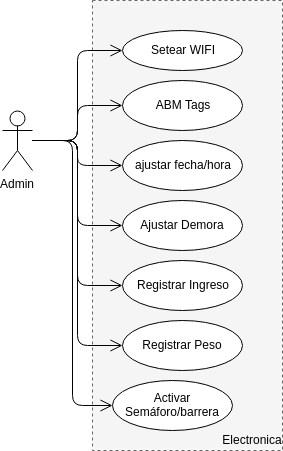
\includegraphics[width=0.5\textwidth]{images/casos_uso_electronica.png}
		\caption{Casos de uso Electr\'onica}
		\label{fig:usecase}
	\end{center}
\end{figure}

\subsection{Secuencia para un registro}
Para registrar un evento se seguir\'a la secuencia demostrada el la figura \ref{fig:sequence-elect}
\begin{figure}[h!]
	\begin{center}
		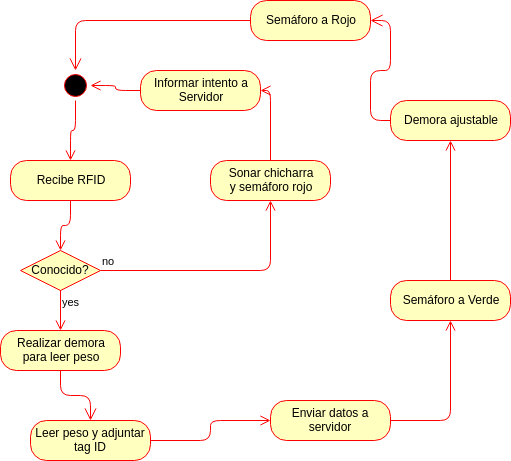
\includegraphics[width=0.7\textwidth]{images/diagrama_secuencia_electronica.png}
		\label{fig:sequence-elect}
		\caption{Diagrama de secuencia}
	\end{center}
\end{figure}

\subsection{Secuencia para agregar un TAG}
La secuencia en la figura \ref{fig:seq-tag} muestra los pasos requeridos para agregar un tag como conocido en la base del equipo, 
los tags que no estén como conocidos causarán una alerta en el sistema y no cambiará el semáforo o activará la barrera.
\begin{figure}[h!]
	\begin{center}
		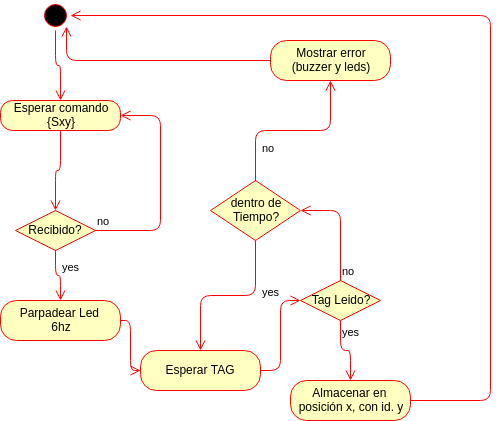
\includegraphics[width=0.6\textwidth]{images/secuencia-agregar-tag.png}
		\caption{Secuencia registro de tag}
		\label{fig:seq-tag}
	\end{center}
\end{figure}

\subsubsection{Dise\~no del PCB}
El dise\~no de la placa para el sistema electr\'onico se detalla en la figura \ref{fig:pcb}
\begin{figure}[h!]
	\begin{center}
		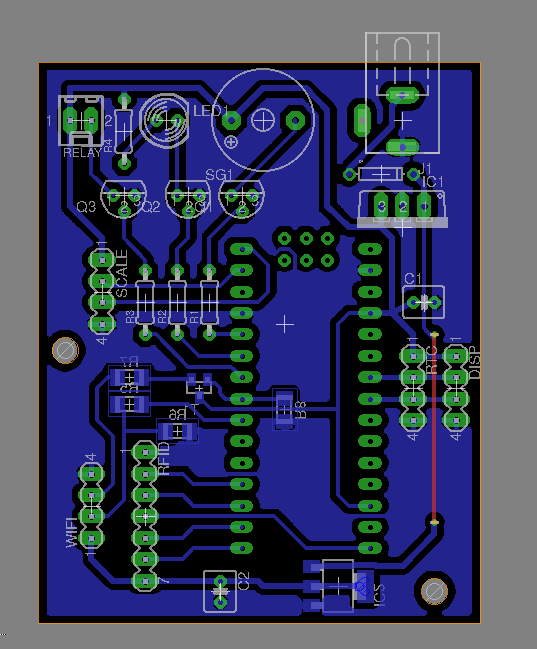
\includegraphics[width=0.5\textwidth]{images/weightlogger_pcb.png}
		\caption{PCB v1.0}
		\label{fig:pcb}
	\end{center}
\end{figure}

Al no disponer de más de una interface serial, la conexión con el wifi y/o balanza (a determinar en pruebas) 
se hará mediante I2C, con la placa mostrada en la figura \ref{fig:pcb-i2c}
\begin{figure}[h!]
	\begin{center}
		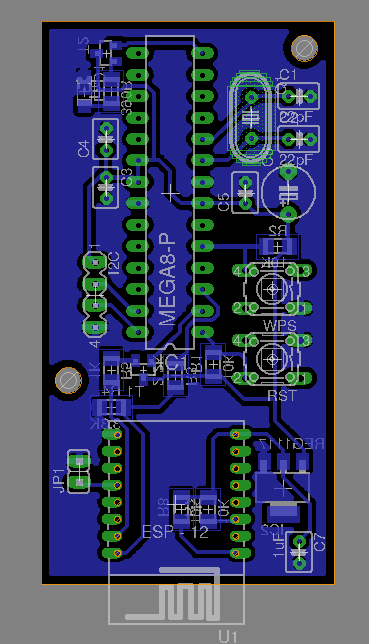
\includegraphics[width=0.5\textwidth]{images/interface-i2c-wifi.png}
		\caption{PCB interface I2C-Serial}
		\label{fig:pcb-i2c}
	\end{center}
\end{figure}

\subsection{Protocolo de comando}
El sistema electrónico entenderá un protocolo de comandos mínimo que le permita ejercer todas sus funciones, para la versión 1.0 del mismo se ha diseñado el siguiente:
\begin{itemize}
	\item TIME-ADJUST: Para permitir el ajuste del rtc incorporado en el equipo.
	\item STORE-CARD: Almacenar tarjeta nueva en posicion determinada.
	\item DUMP-EEPROM: Descargar el contenido de la eeprom interna con los tags conocidos.
	\item ERASE-CARD: Borrar un tag conocido de la memoria EEPROM.
	\item REJECTED: Envío de un intento de ingreso rechazado.
	\item RECORD: Envío de un registro completo con peso, fecha/hora y TAG ID.
\end{itemize}
Este protocolo mínimo será soportado por la versión 1.0 y se recibirá mediante protocolo TCP/IP por la red inalámbrica. El detalle de los bytes enviados y respuesta se detallará a continuación.

\begin{itemize}
	\item[TIME-ADJUST] [Twxyz] el comando comienza con la letra T mayúscula acompañado de 4 bytes que representan el tiempo en formato unix timestamp, comenzando por el LSB hacia el MSB\label{itm:ta}.
	\item[STORE-CARD] [Sxy] Comando de letra S mayúscula acompañado de dos bytes, \emph{x} para posición de 0 a 200, \emph{y} para identificador de tag que será exportado al enviar registro. El ID del tag a guardar será leido por el dispositivo.\label{itm:sc}
	\item[DUMP-EEPROM] [D0] Comando de letra D mayúscula, no requiere parámetro adicional.
	\item[ERASE-CARD] [Ex] Comando de letra E mayúscula, acompañado de byte \emph{x} con la posición a borrar, de 0 a 200.
	\item[REJECTED] [Rwxyzabcd] Comando con letra R mayúscula, acompañado de los 4 bytes de unixtimestamp como en TA\footnote{TIME-ADJUST} y 4 bytes del TAG ID rechazado.
	\item[RECORD] [Awxyzabcdefgi] Comando con la letra A mayúscula, acompañado de los 4 bytes de unixtimestamp igual que en TA, los siete bytes del peso leídos de la báscula y el ID del tag leido en el último byte.
\end{itemize}

\subsection{Mensajes del sistema}
El dispositivo electrónico contará con mensajes que mostrará a travez de su display, los mismos se detallan a continuación:
\begin{itemize}
	\item En modo espera mostrará ``Esperando'' y la hora y fecha actual.
	\item Al recibir un tag conocido mostrará: ``Acceso permitido''.
	\item Cuando lea un tag desconocido mostrará: ``Acceso negado, informando''.
	\item Al confirmar pesaje o luego de la demora mostrará ``Avance...''.
	\item En Configuración mostrará el IP obtenido por el wifi. 
	\item En caso de error mostrará ``Error'' y un código detallado en la sección \ref{sec:errores}
\end{itemize}

\subsubsection{Códigos de error}
Los siguientes códigos de error se manejarán en el dispositivo:\label{sec:errores}\\
\begin{center}
	\begin{tabular}{|c|l|}
		\hline
		Código & Descripción \\
		\hline
		501 & Falla RTC\\
		502 & Falla RFID\\
		503 & Falla WiFi\\
		504 & Falla EEPROM\\
		\hline
	\end{tabular}
\end{center}
\subsection{Software de Administración}

El software de administraci\'on requerido ser\'a desarrollado en Ruby On Rails para mejor velocidad de desarrollo.

\subsubsection{Casos de uso para el sistema}
Los casos de uso que se han considerado para el sistema administrativo se detallan en la figura \ref{fig:usecase-admin}, se incorporarán más casos en las subsiguientes iteraciones del sistema.
\begin{figure}[h!]
	\begin{center}
		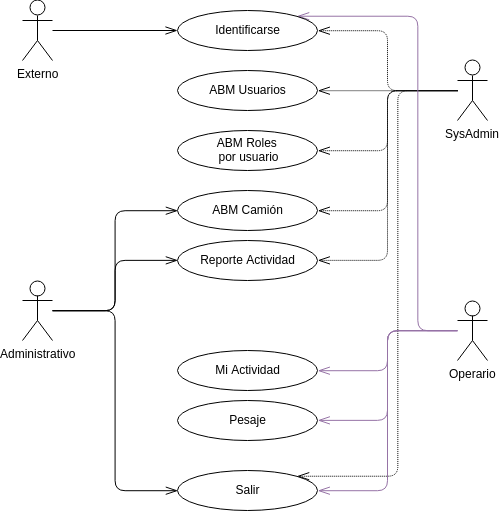
\includegraphics[width=0.6\textwidth]{images/casos-sistema-admin.png}
		\caption{Casos de uso sistema Administrativo}
		\label{fig:usecase-admin}
	\end{center}
\end{figure}

\subsubsection{Diagrama de entidad relación}
Las entidades y sus relaciones se detallan en la figura \ref{fig:er}, se evolucionarán sus partes acorde se avance en las versiones del sistema desarrollado.
\begin{figure}[h!]
	\begin{center}
		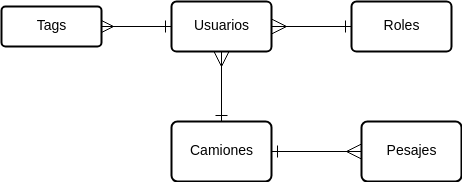
\includegraphics[width=0.6\textwidth]{images/ER-SistemaAdmin.png}
		\caption{Diagrama Entidad-Relación}
		\label{fig:er}
	\end{center}
\end{figure}

\subsubsection{Desiciones de diseño del sistema admin}

Se utilizará la mayor cantidad de gemas disponibles para el sistema, de forma tal que ascelere el desarrollo y se pueda entregar rápidamente algo de utilidad al cliente final.

Utilizaremos al menos las siguientes gemas:
\begin{itemize}
	\item Devise, para manejo de autentificación.
	\item ActiveAdmin, para ABMs rápidos.
	\item etc.
\end{itemize}